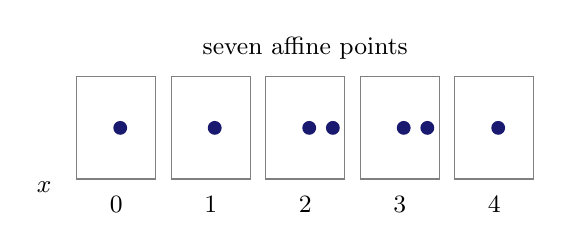
\begin{tikzpicture}[font=\small]
\foreach \x/\n/\v in {0/0/1,1.2/1/1,2.4/2/2,3.6/3/2,4.8/4/1}{
\draw[gray] (\x,0) rectangle +(1,1.3);
\node[below] at (\x+.5,-.1) {$\n$};
\foreach \j in {1,...,\v}{\fill[MidnightBlue] (\x+.25+.3*\j,.65) circle(2.5pt);}
}
\node[left] at (-.2,-.1) {$x$};
\node[above] at (2.9,1.4) {seven affine points};
\end{tikzpicture}
